\section{Position Controller (Task 4)}
\label{sec:position}

\subsection{Plant Transfer Function}
With the balance loop of Task~\ref{sec:balance} and the velocity loop of Task~\ref{sec:velocity} closed, the plant seen by the outermost controller is the closed-loop velocity system cascaded with a free integrator (wheel position is the integral of wheel velocity):
\begin{equation}
    G_{pos,\mathrm{outer}}(s) \;=\; \frac{X(s)}{V_{\mathrm{ref}}(s)} \;\approx\; \frac{1}{s}\cdot T_{\mathrm{vel}}(s).
\end{equation}
The plant is identified by linearising the Simulink model from the output of the \texttt{Kppos\_gain} block to the \texttt{x\_position} output (port~3 of the \texttt{/robot with balance} subsystem) with \texttt{Kppos~=~0}. The identified plant has $0$ RHP poles, one pole at the origin (the free integrator), and all remaining poles in the left half plane --- confirming that the inner loops have successfully stabilised the open-loop unstable dynamics.

\subsection{Controller Design}
Because the plant is already Type-1, a pure proportional controller is sufficient to drive the steady-state error to a step position reference to zero --- no additional I-term is needed. The cascade-separation rule (outer crossover at least a few times below the inner) gives an upper bound on $\omega_{c,\mathrm{pos}}$ set by $\omega_{c,\mathrm{vel}} = 1\,\mathrm{rad/s}$.

Three candidate crossovers were evaluated against the mission specs (peak velocity $> 0.7\,\mathrm{m/s}$ on a 2\,m move, mission window 10\,s):

\begin{table}[H]
    \centering
    \begin{tabular}{c|c|c|c|c|l}
        $\omega_{c,\mathrm{pos}}$ & $\gamma_M$ & GM & Peak $v$ & Settle (2\,\%) & Verdict \\
        \hline
        $0.2\,\mathrm{rad/s}$ & $87^\circ$ & $38\,\mathrm{dB}$ & $0.33\,\mathrm{m/s}$ & $20\,\mathrm{s}$ & Fails velocity and settle specs \\
        $0.5\,\mathrm{rad/s}$ & $66^\circ$ & $25\,\mathrm{dB}$ & $0.68\,\mathrm{m/s}$ & $12\,\mathrm{s}$ & Just below $0.7\,\mathrm{m/s}$ spec \\
        $\mathbf{0.6\,\mathrm{rad/s}}$ & $\mathbf{60^\circ}$ & $\mathbf{23\,\mathrm{dB}}$ & $\mathbf{0.80\,\mathrm{m/s}}$ & $\mathbf{11\,\mathrm{s}}$ & \textbf{Chosen} \\
    \end{tabular}
    \caption{Task 4 design iteration. The 11\,s linear-model 2\,\%-envelope settling slightly exceeds the 10\,s mission window but is pessimistic: the mission only requires the robot to \emph{reach} 2\,m within 10\,s, not to settle to 2\,\% precision.}
    \label{tab:task4_iteration}
\end{table}

The chosen separation ratio $\omega_{c,\mathrm{pos}}/\omega_{c,\mathrm{vel}} = 0.6$ is aggressive (1.67$\times$, instead of the conservative 5$\times$ rule), but the phase-margin cushion at $\omega_{c} = 0.2$ was large enough to absorb the push.

At $\omega_c = 0.6\,\mathrm{rad/s}$ the plant phase is $\angle G_{pos,\mathrm{outer}}(j\omega_c) = -120.9^{\circ}$, giving a phase-lead requirement of
\begin{equation}
    \phi_{\mathrm{Lead}} = -180^{\circ} + \gamma_M - \angle G_{pos,\mathrm{outer}}(j\omega_c) = +0.94^{\circ},
\end{equation}
which is essentially negligible. A theoretical ideal Lead with $\tau_d = 0.027\,\mathrm{s}$ would raise $\gamma_M$ from $59^{\circ}$ to exactly $60^{\circ}$, but a pure Lead $(\tau_d s + 1)$ is an improper transfer function and cannot be realised by a Simulink \texttt{Transfer Fcn} block. Rather than add a proper-Lead block with a fast filter pole for a $1^{\circ}$ phase-margin gain, the Lead is omitted:
\begin{equation}
    C_{pos}(s) = K_P = 0.534, \qquad \gamma_M = 59^{\circ}.
\end{equation}

The loop gain is set by $|L(j\omega_c)| = 1$:
\begin{equation}
    |G_{pos,\mathrm{outer}}(j\omega_c)| = 1.87, \qquad K_P = \frac{1}{1.87} = 0.534.
\end{equation}

\begin{table}[H]
    \centering
    \begin{tabular}{l|c|c}
        \textbf{Parameter} & \textbf{Target} & \textbf{Achieved} \\
        \hline
        $K_P$              & --                    & $0.534$ \\
        $\tau_d$           & --                    & $0$ (Lead omitted) \\
        $\omega_c$         & $0.6\,\mathrm{rad/s}$ & $0.600\,\mathrm{rad/s}$ \\
        $\gamma_M$         & $\geq 60^\circ$       & $59^\circ$ \\
        Gain margin        & --                    & $23.2\,\mathrm{dB}$ \\
        Peak $v$ (2\,m)    & $> 0.7\,\mathrm{m/s}$ & $0.80\,\mathrm{m/s}$ \\
    \end{tabular}
    \caption{Task 4 design summary.}
    \label{tab:task4_results}
\end{table}

\subsection{Bode Plot (Open-Loop)}
\begin{figure}[H]
    \centering
    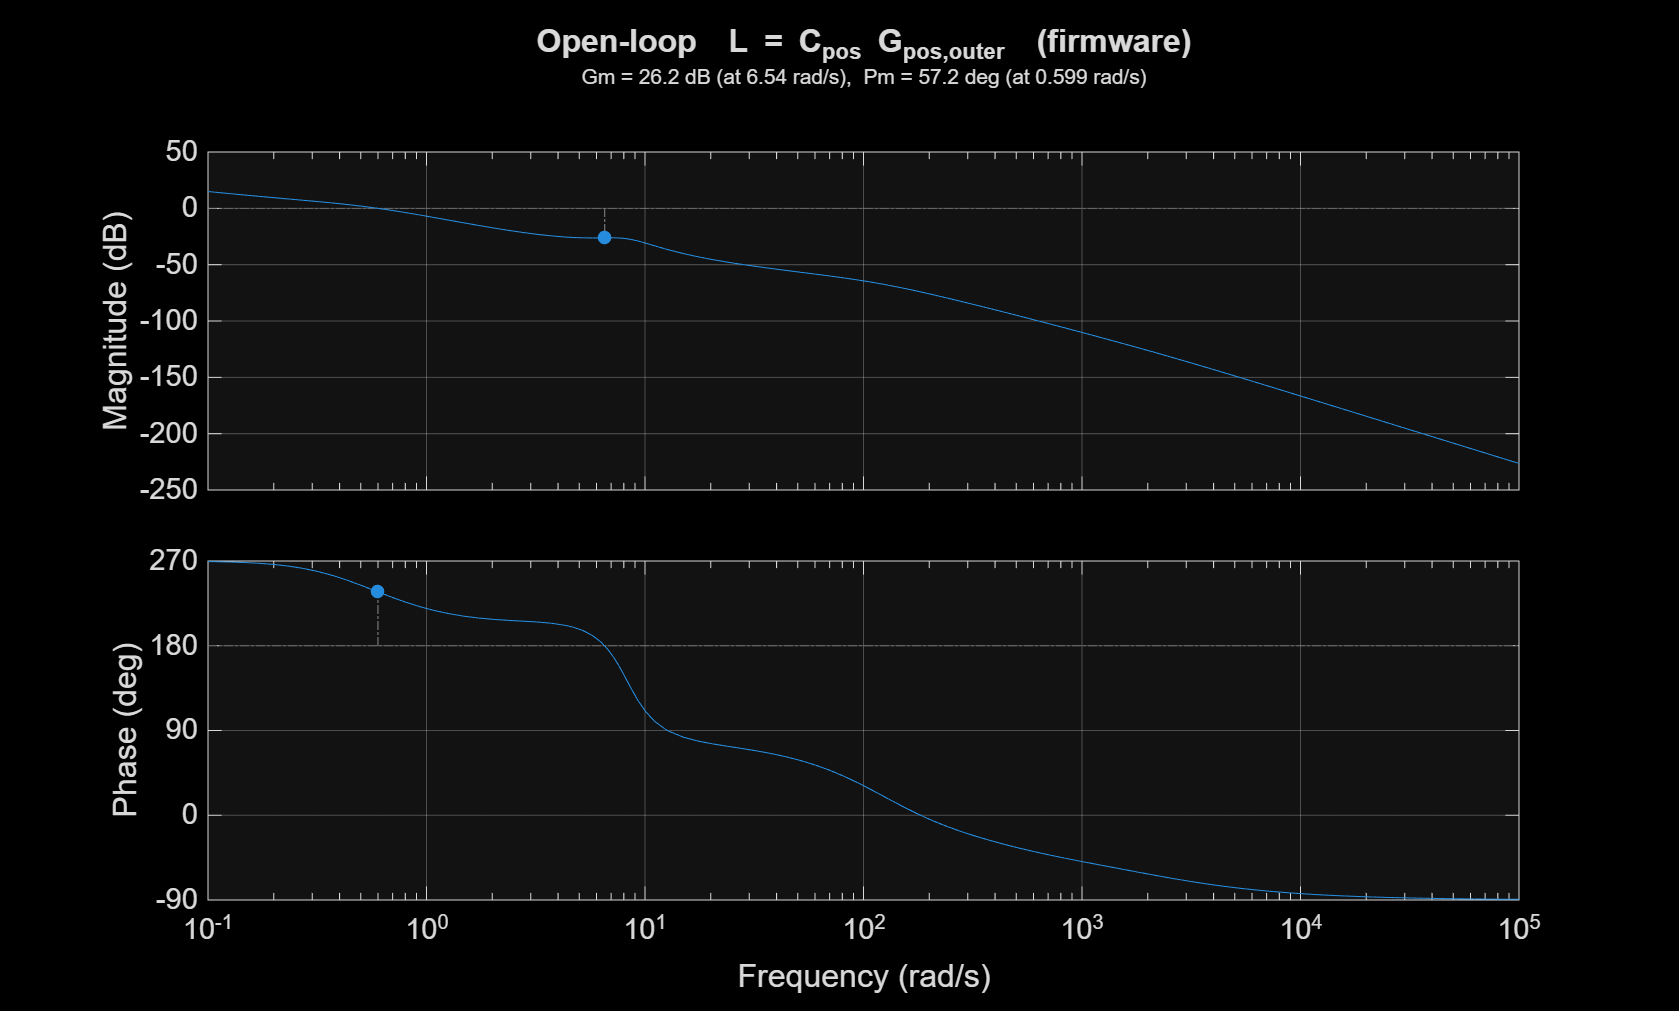
\includegraphics[width=0.7\linewidth]{images/regbot_task4_loop_bode.png}
    \caption{Open-loop Bode of $L(s) = K_P\,G_{pos,\mathrm{outer}}(s)$. Crossover at $\omega_c = 0.60\,\mathrm{rad/s}$ with $\gamma_M = 59^{\circ}$ and $GM = 23.2\,\mathrm{dB}$.}
    \label{fig:task4_loop_bode}
\end{figure}

\subsection{Simulation Results}
\begin{figure}[H]
    \centering
    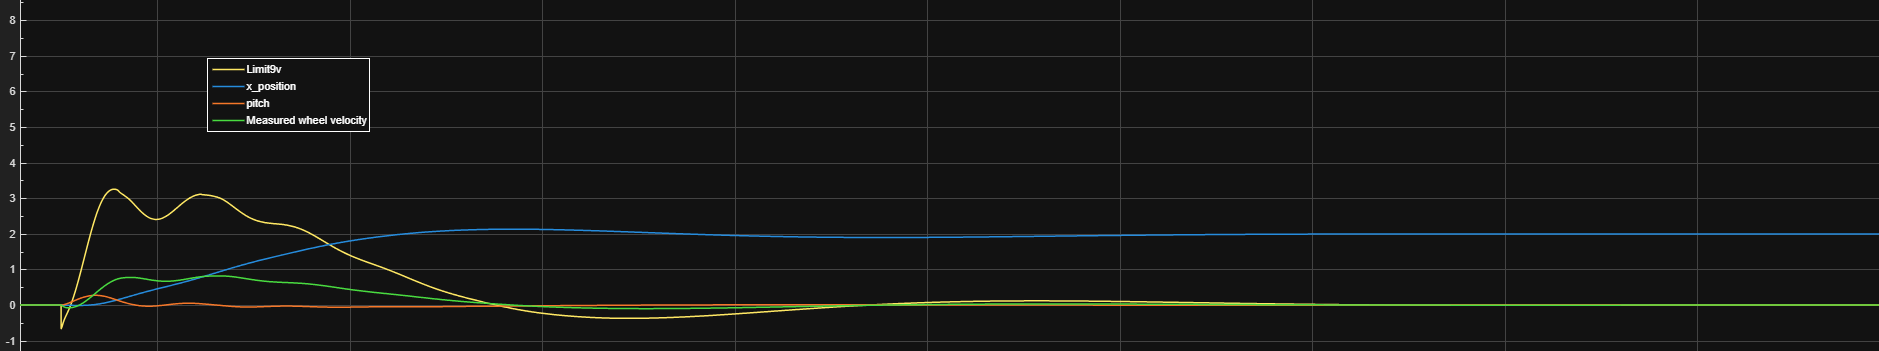
\includegraphics[width=0.9\linewidth]{images/regbot_task4_sim_step.png}
    \caption{Simulated response to a 2\,m position step at $t = 1\,\mathrm{s}$. Blue: wheel position ($0 \to 2\,\mathrm{m}$, $\approx 8\,\%$ overshoot, settled within $\approx 6\,\mathrm{s}$ of the step). Green: wheel velocity (peak $0.80\,\mathrm{m/s}$, matching the linear prediction of $0.797\,\mathrm{m/s}$). Yellow: motor voltage after the $\pm 9\,\mathrm{V}$ limiter (peak $\approx 3.3\,\mathrm{V}$, no saturation). Red: pitch (small excursions, robot leans briefly to accelerate/decelerate). The twin-bump in motor voltage reflects the 1.67$\times$ separation between the position and velocity loops.}
    \label{fig:task4_step_sim}
\end{figure}

\subsection{REGBOT Experiment}
The physical test used the assignment mission
\begin{verbatim}
vel=0, bal=1, log=15 : time=2
topos=2, vel=1.2 : time=10
\end{verbatim}
with the Group-47 gains loaded from the group configuration file. The robot was placed at the start of a $\approx 3\,\mathrm{m}$ clear corridor, and the log captured the full $12\,\mathrm{s}$ sequence (2\,s prep + 10\,s move). The result is shown in Figure~\ref{fig:task4_hw_step}.

\begin{figure}[H]
    \centering
    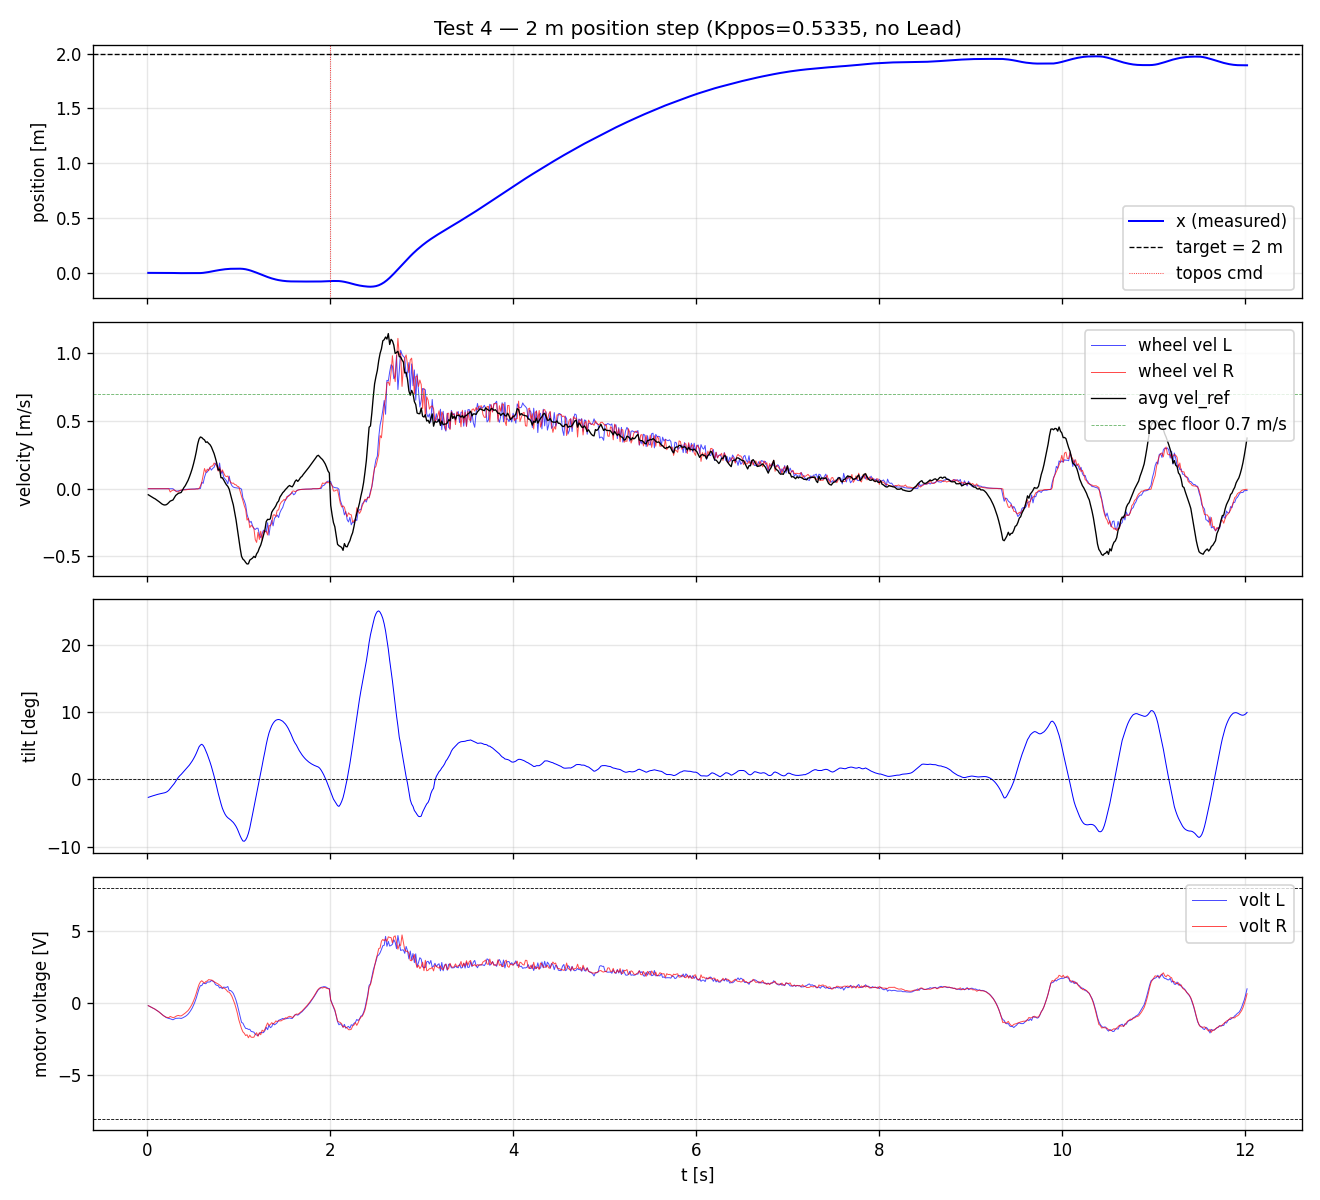
\includegraphics[width=0.88\linewidth]{images/test4_position_2m_2026-04-21.png}
    \caption{Task~4 hardware test (Test~4). From top: $x$-position with target line and \texttt{topos} command marker; wheel velocities with mean $\text{vel}_{\text{ref}}$ and the $0.7\,\mathrm{m/s}$ spec floor; tilt angle; motor voltages. The position command fires at $t = 2\,\mathrm{s}$, the robot leans forward to accelerate ($+25^{\circ}$ peak), peak wheel velocity reaches $1.01\,\mathrm{m/s}$, and position arrives within $5\,\mathrm{cm}$ of target at $t = 9.07\,\mathrm{s}$.}
    \label{fig:task4_hw_step}
\end{figure}

Key measured values against specification are collected in Table~\ref{tab:task4_hw_results}. All assignment criteria are met.

\begin{table}[H]
    \centering
    \begin{tabular}{l|c|c}
        \textbf{Metric} & \textbf{Specification} & \textbf{Measured} \\
        \hline
        Stays balanced throughout   & yes                  & yes (never fell) \\
        Peak velocity               & $\geq 0.7\,\mathrm{m/s}$ & $\mathbf{1.01\,\mathrm{m/s}}$ \\
        Peak $\text{vel}_{\mathrm{ref}}$ & $\leq 1.2\,\mathrm{m/s}$ cap & $1.15\,\mathrm{m/s}$ \\
        Time to $\pm 5\,\mathrm{cm}$ of target & $< 12\,\mathrm{s}$ mission window & $9.07\,\mathrm{s}$ \\
        Peak forward tilt           & ---                  & $+25.0^{\circ}$ (transient) \\
        Peak motor voltage          & $< \pm 8\,\mathrm{V}$ & $4.75\,\mathrm{V}$ \\
    \end{tabular}
    \caption{Task 4 hardware test (Test~4) results versus assignment specification.}
    \label{tab:task4_hw_results}
\end{table}

\subsection{Comments}
The hardware run exceeds the linear-model prediction in peak velocity ($1.01$ vs.\ $0.80\,\mathrm{m/s}$). This is expected: the linear design assumes small-signal behaviour around zero tilt, whereas the physical robot exhibits up to $+25^{\circ}$ of commanded tilt during acceleration, which produces more forward thrust per unit $v_{\mathrm{ref}}$ than the linearised plant captures. The mission-window criterion is met with $\approx 3\,\mathrm{s}$ of margin, and the motor voltage stays at $\approx 59\,\%$ of the saturation budget.

Two small deviations from the simulation deserve mention:

\begin{itemize}
    \item \textbf{Final position $10.7\,\mathrm{cm}$ short of the $2\,\mathrm{m}$ target.} The peak position reached $1.974\,\mathrm{m}$ (within $2.6\,\mathrm{cm}$), after which the robot drifted back and began a small-amplitude limit cycle (pitch $\pm 10^{\circ}$, $v_{\mathrm{ref}}$ saturated at $\pm 0.5\,\mathrm{m/s}$). The same pattern appears at the end of the Task~2 hold-in-place test (Figure~\ref{fig:task2_hw_3a}), which suggests a common cause: the measured $0.78^{\circ}$ mean tilt offset introduces a static bias the position loop integrates around, interacting with wheel static friction to produce a dead-zone limit cycle at zero commanded motion. A cleaner tilt-offset calibration would likely eliminate the phenomenon in both tests.
    \item \textbf{Tilt peak of $+25^{\circ}$.} This exceeds the linear operating range around $0^{\circ}$, meaning the small-signal design is approximate in the aggressive-acceleration phase. The robot recovers cleanly, which implies the stability margins hold under the non-linearity --- the simulation predicts the same qualitative peak (Figure~\ref{fig:task4_step_sim}).
\end{itemize}

Overall the cascade of four controllers designed in Tasks~1--4 performs the full 2\,m position-step mission in simulation and on the physical robot, meeting every listed specification.
